\chapter{Выделение краёв}
\label{ch:chap4}

\definecolor{codegreen}{rgb}{0,0.6,0}
\definecolor{codegray}{rgb}{0.5,0.5,0.5}
\definecolor{codepurple}{rgb}{0.58,0,0.82}
\definecolor{backcolour}{rgb}{0.95,0.95,0.92}

\lstdefinestyle{mystyle}{
    backgroundcolor=\color{backcolour},   
    commentstyle=\color{codegreen},
    keywordstyle=\color{magenta},
    numberstyle=\tiny\color{codegray},
    stringstyle=\color{codepurple},
    basicstyle=\ttfamily\footnotesize,
    breakatwhitespace=false,         
    breaklines=true,                 
    captionpos=b,                    
    keepspaces=true,                 
    numbers=left,                    
    numbersep=5pt,                  
    showspaces=false,                
    showstringspaces=false,
    showtabs=false,                  
    tabsize=2
}
\lstset{style=mystyle}

Для следующего задания идеально подойдёт какая-нибудь pixel-art картинка, ведь в них идеально можно понять где края, 
картинка то из больших пикселей состоит...

\begin{figure}[ht]
    \centering
    
\includegraphics[width=0.5\textwidth]{pixel_art_manime.png}
	\caption{Оригинал}
\end{figure}

Для того, чтобы выделить края изображения, нам надо воспользоваться соответствующим ядром:
$$
    edge = \begin{pmatrix}
        -1 & -1 & -1 \\
        -1 & 8 & -1 \\
    -1 & -1 & -1 
    \end{pmatrix}
$$

\section{Через свёртку напрямую}
Делаем свёртку исходного изображения c матрицей ядра для, после нормируем результат от 0 до 1, получаем следующие результаты:

\begin{figure}[ht]
    \centering
    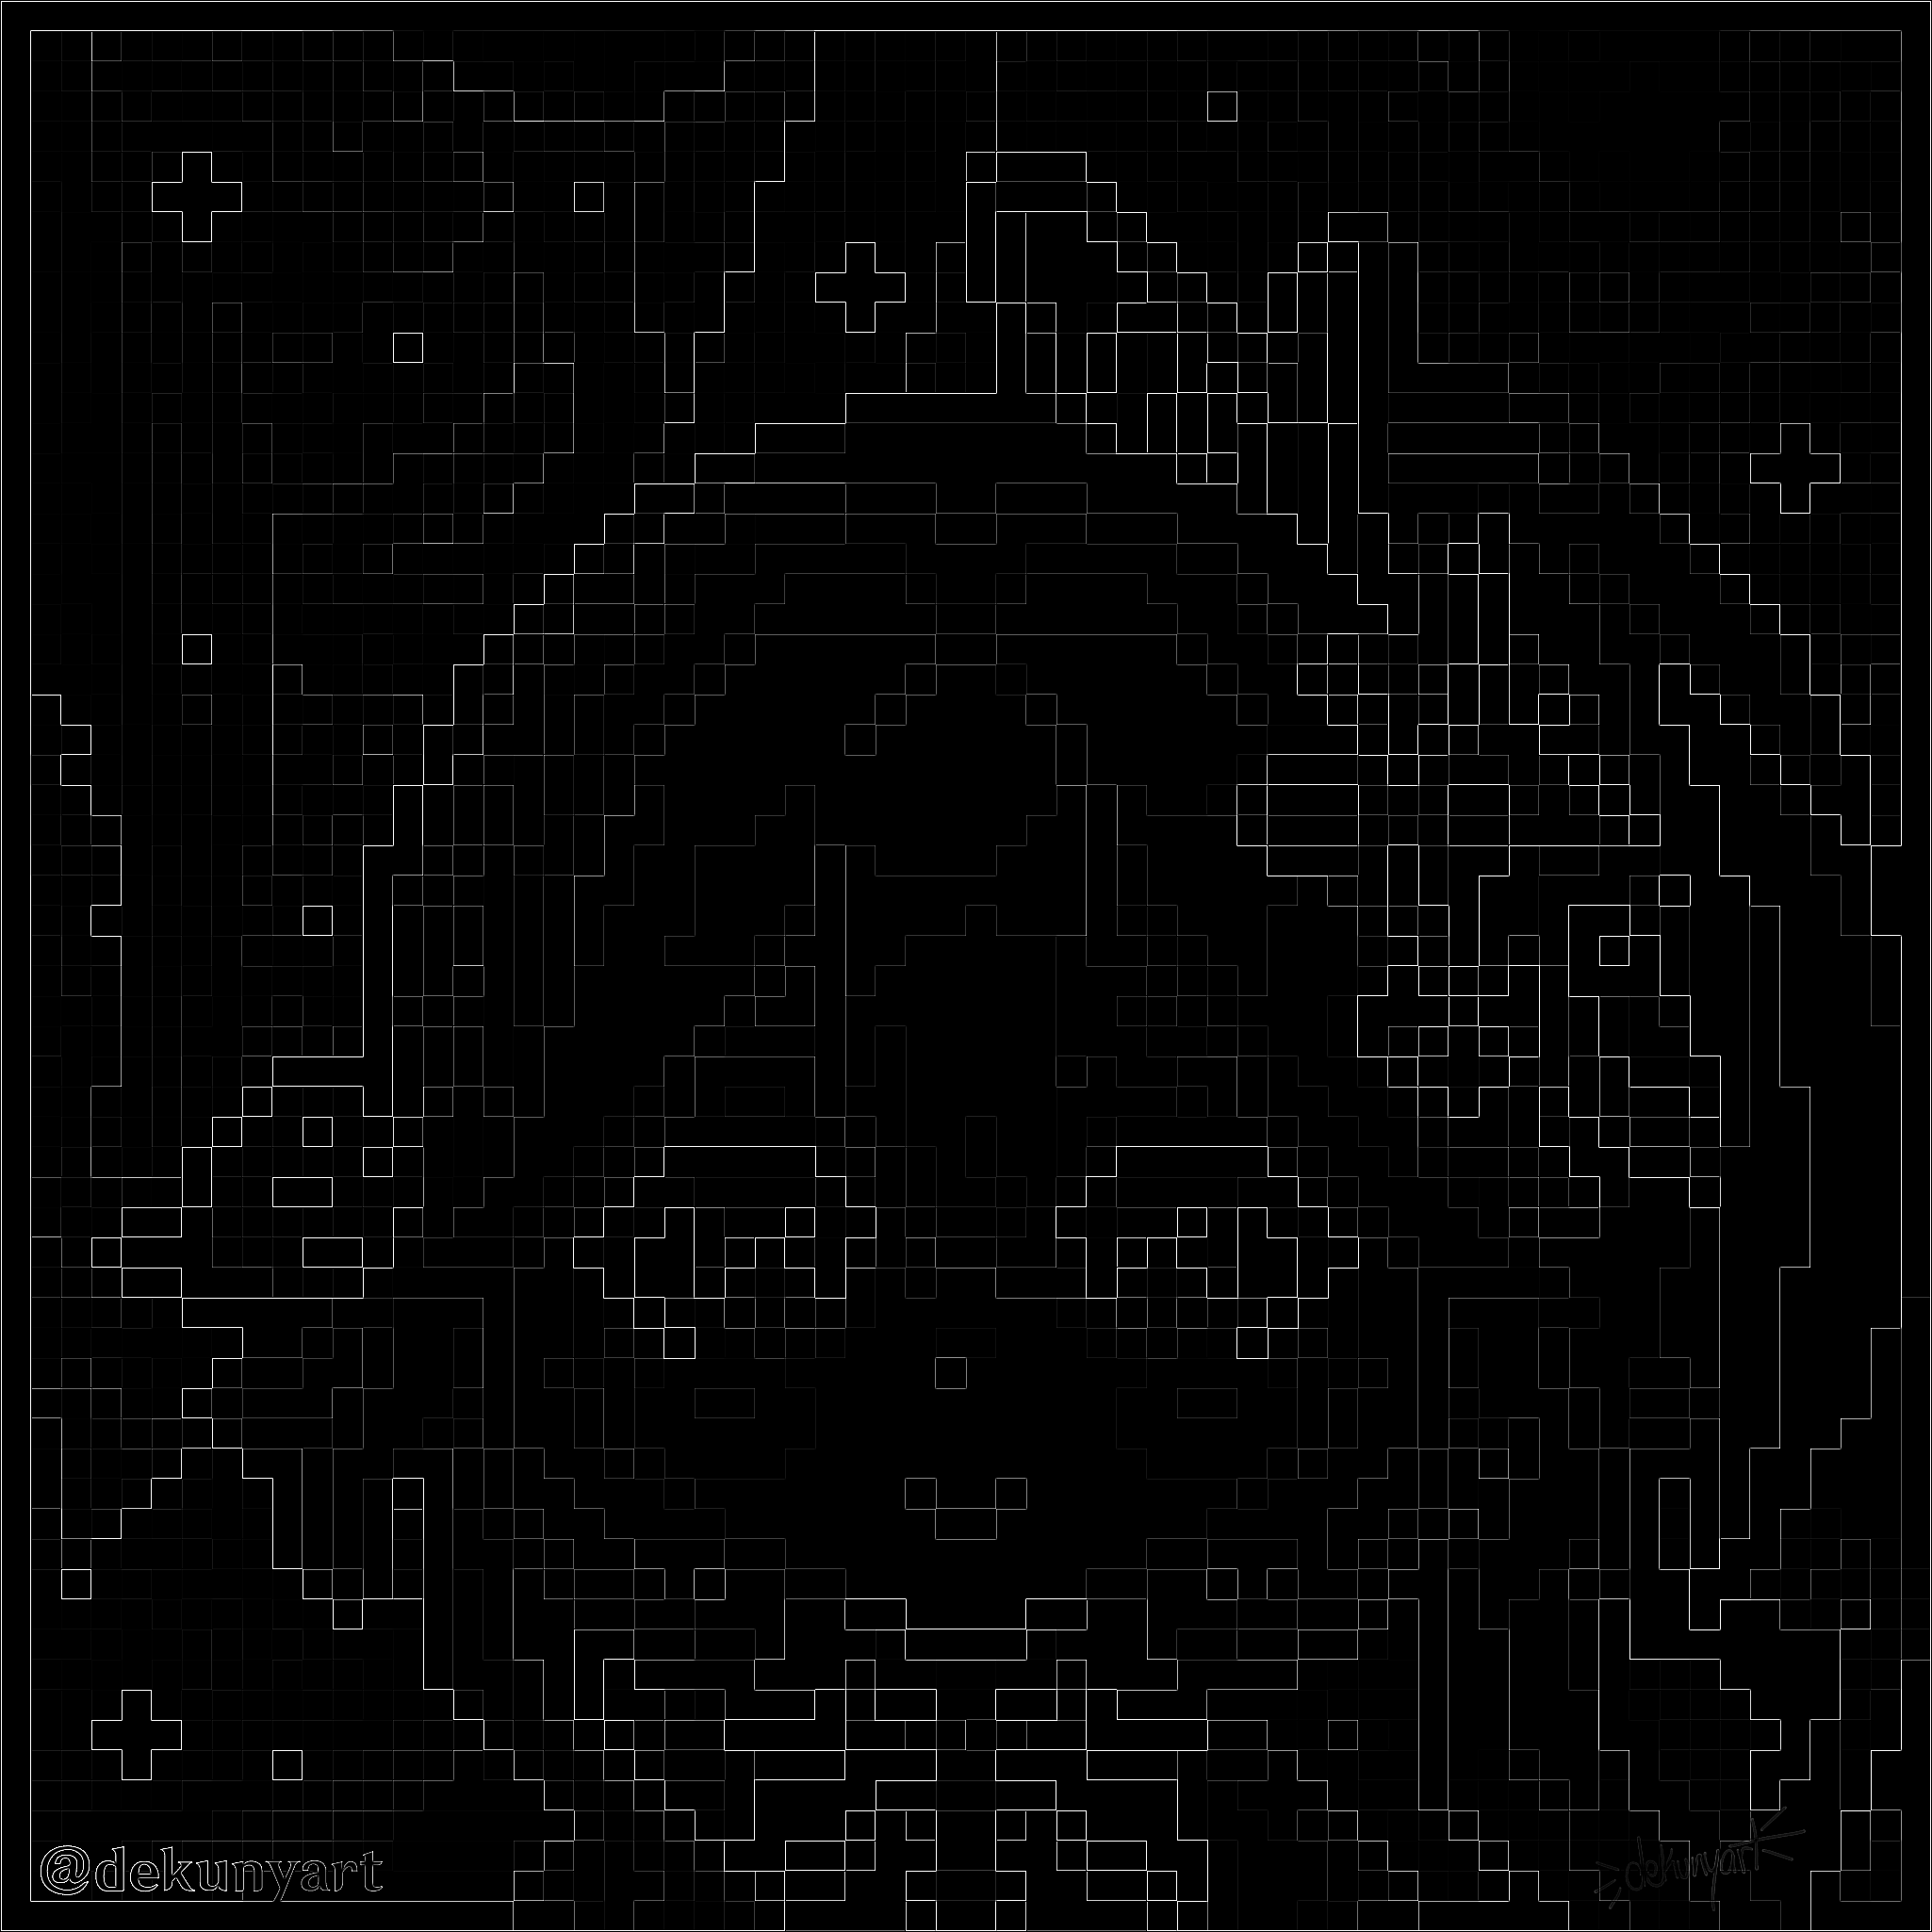
\includegraphics[width=0.6\textwidth]{pixel_art_EDGE1.png}
	\caption{Выделяем края, применили один раз}
\end{figure}



\begin{figure}[ht]
    \centering
    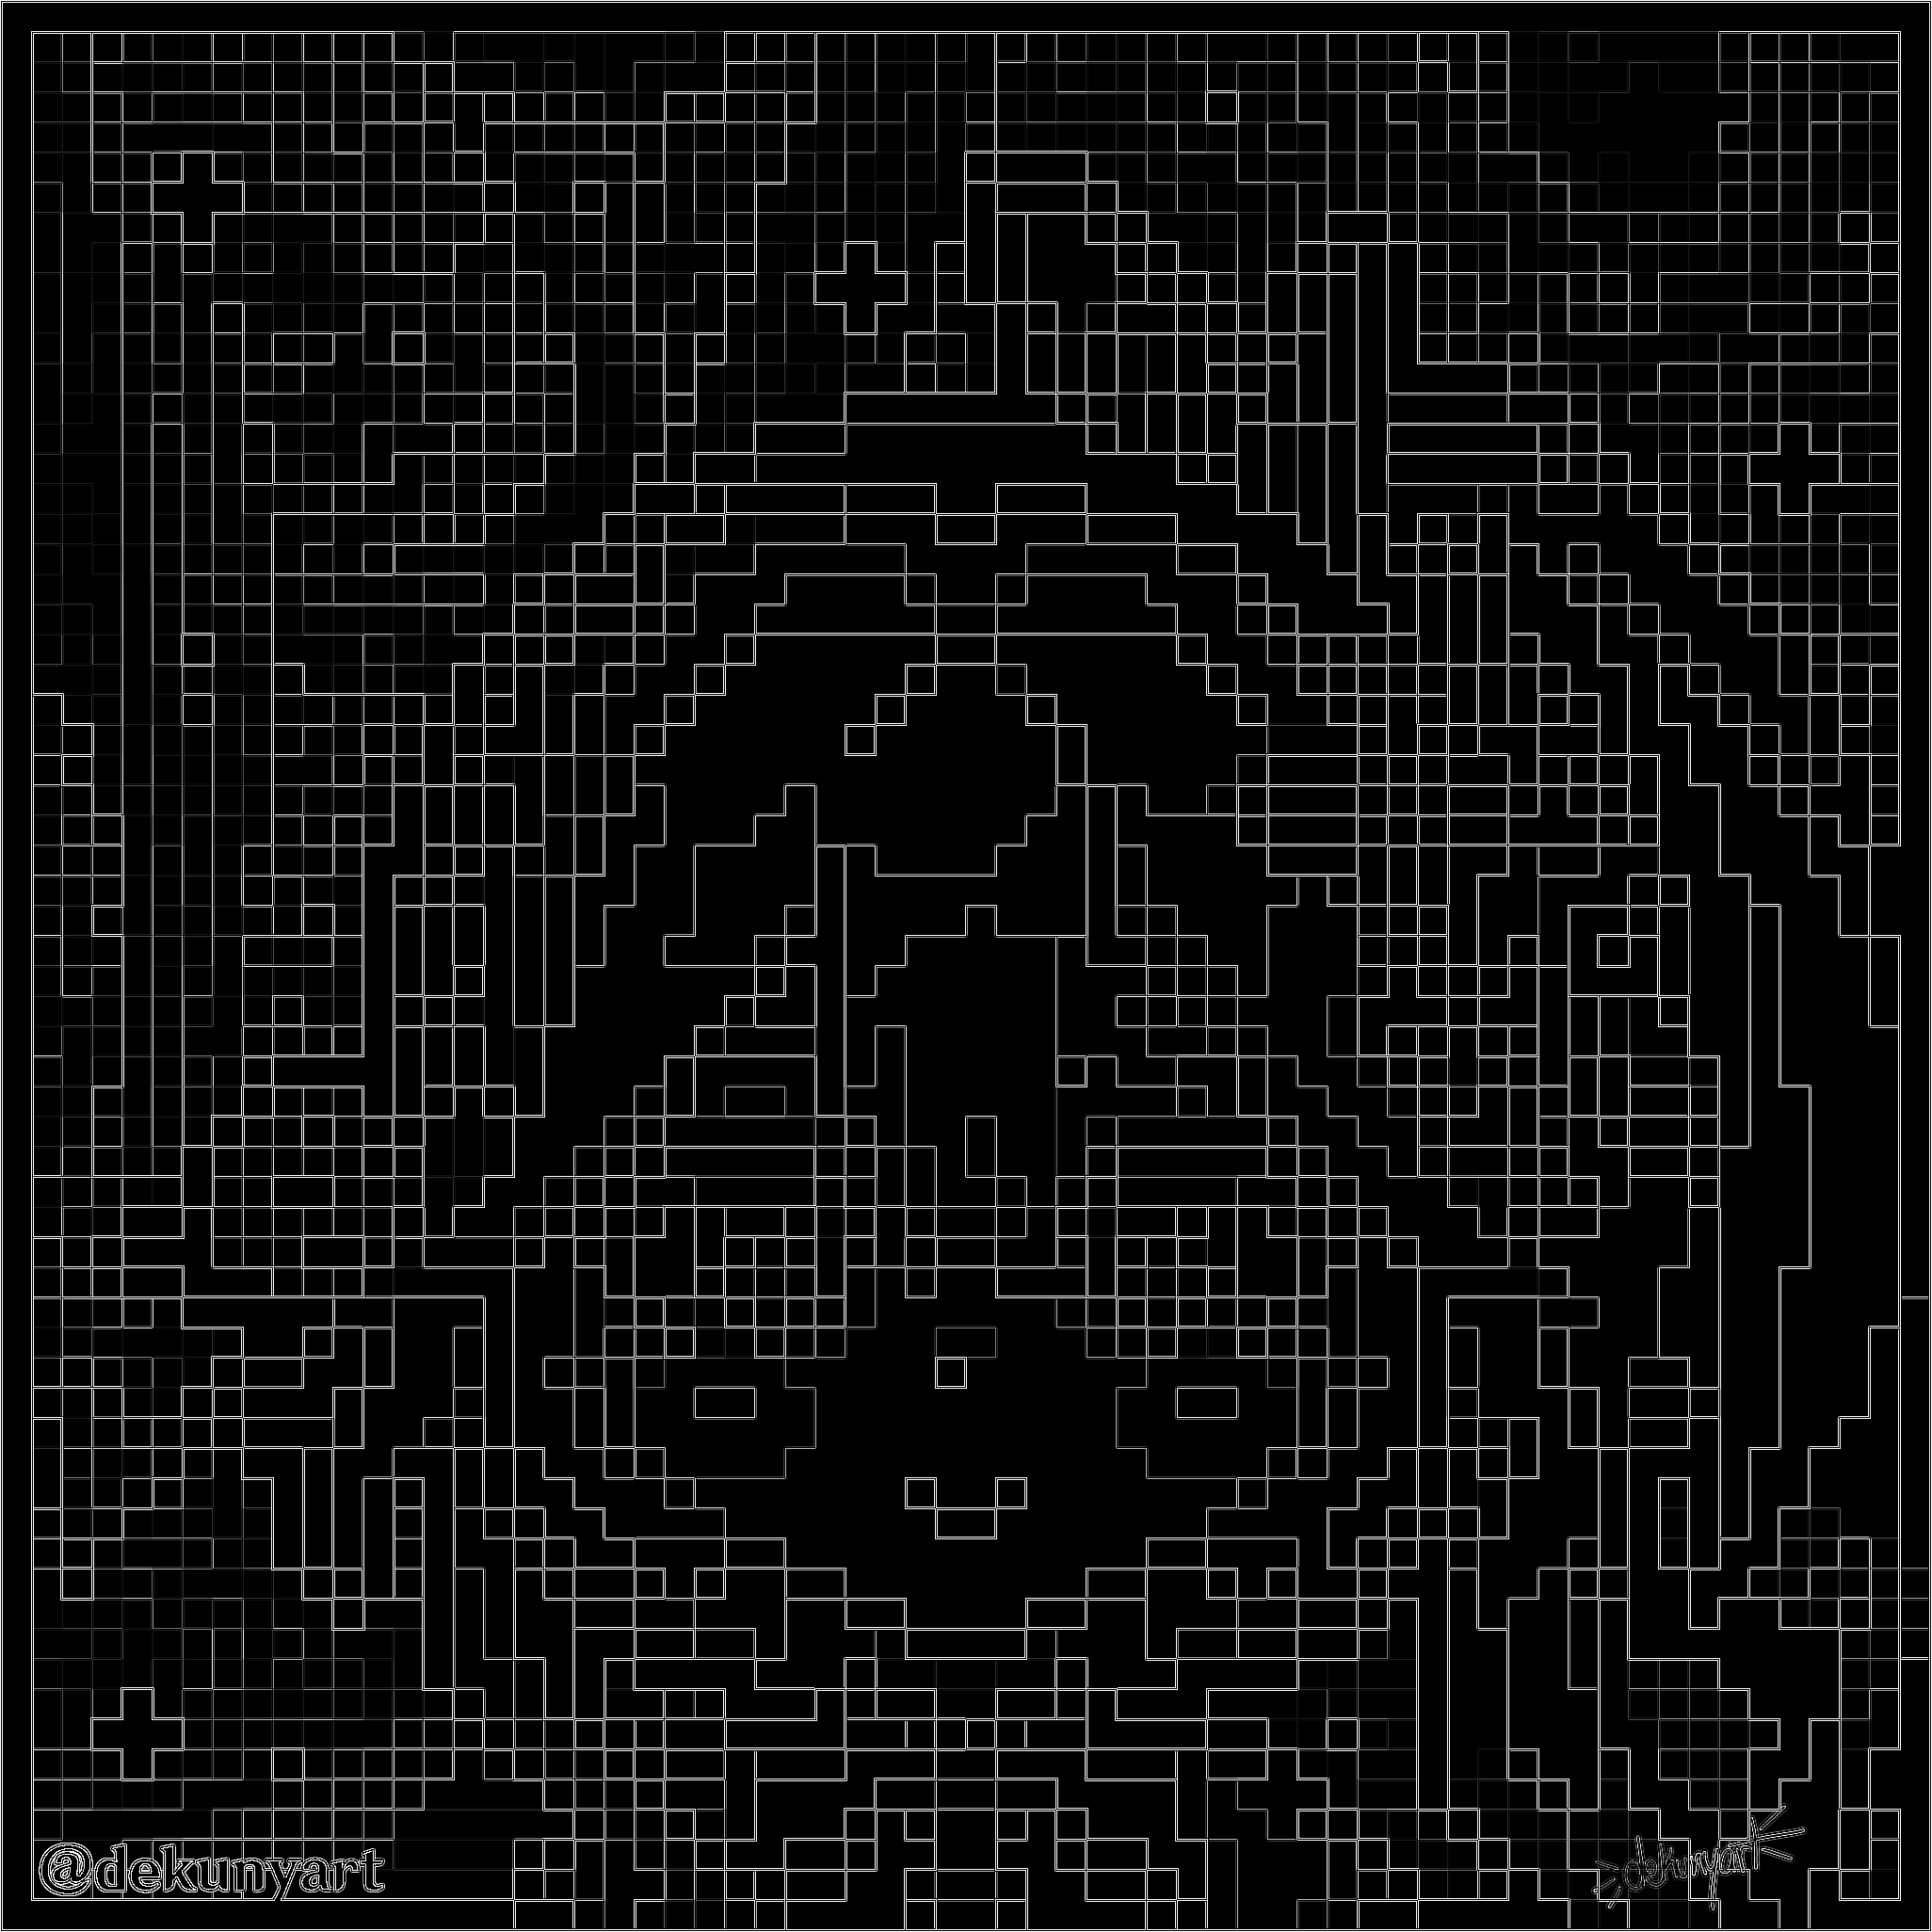
\includegraphics[width=0.6\textwidth]{pixel_art_EDGE2.png}
	\caption{Выделяем края, применили два раза}
\end{figure}


\begin{figure}[ht]
    \centering
    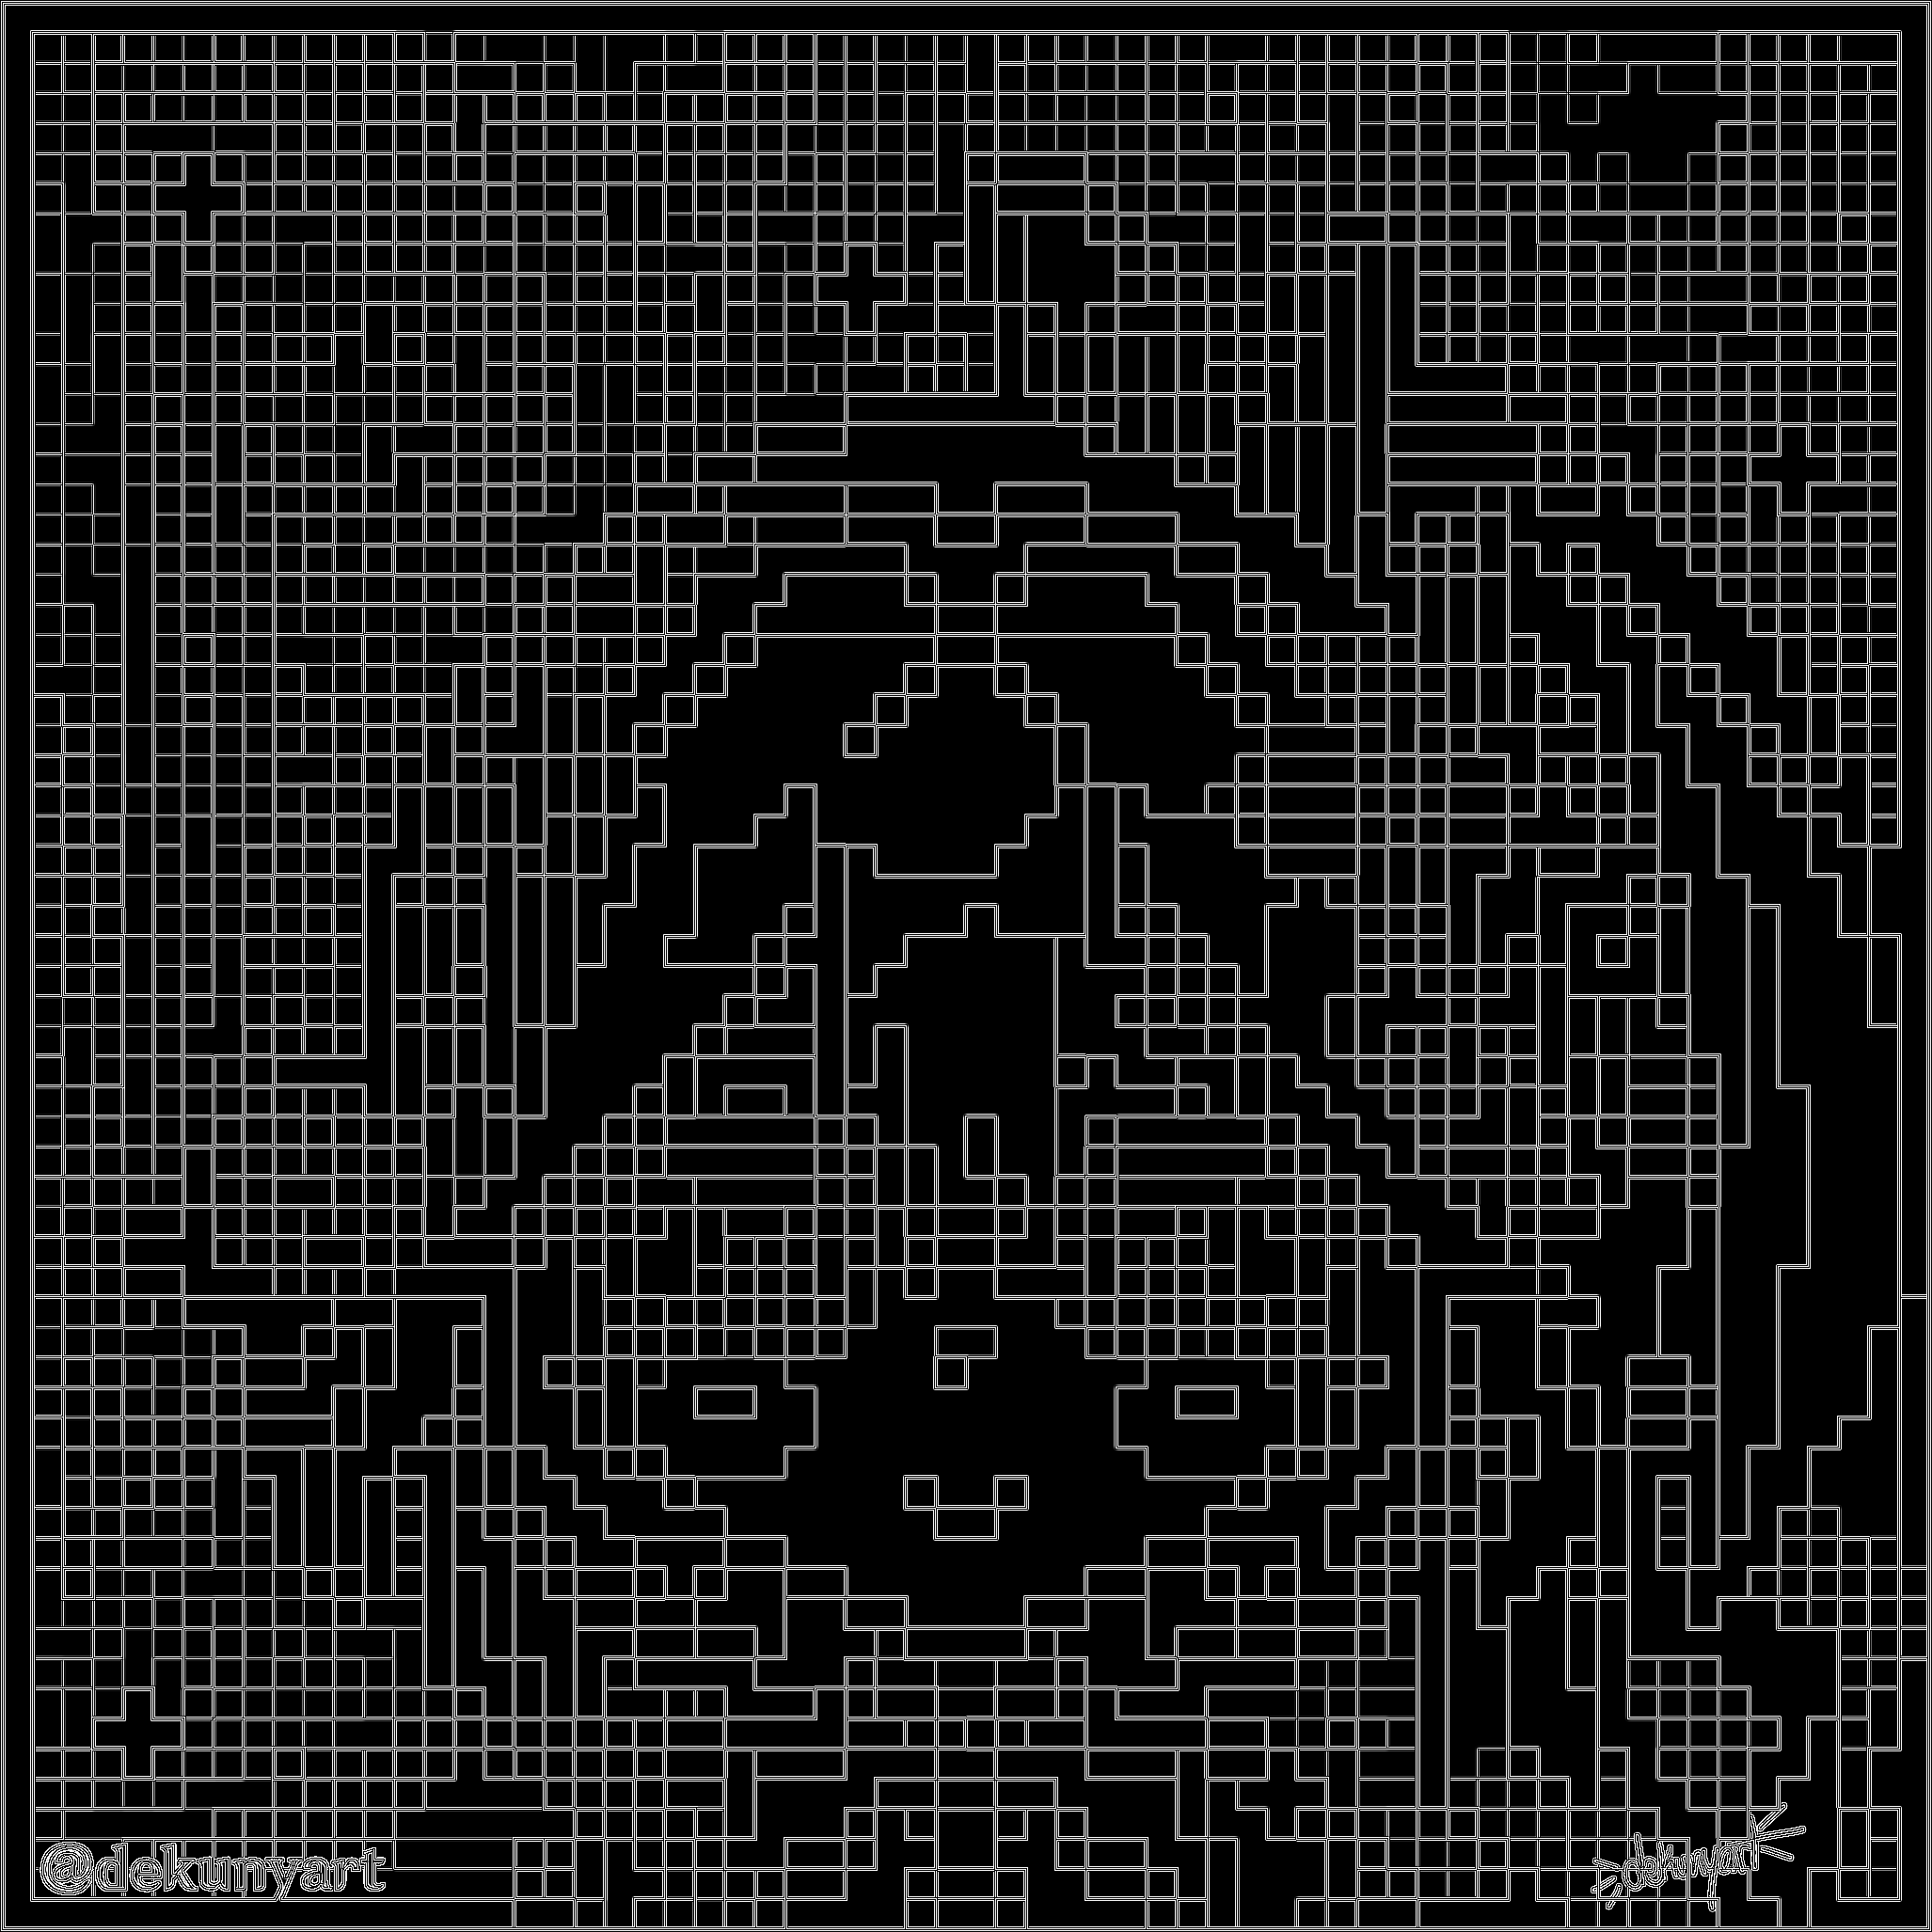
\includegraphics[width=0.6\textwidth]{pixel_art_EDGE3.png}
	\caption{Выделяем края, применили три раза}
\end{figure}

Как можно заметить,  выделение краёв позволяет нам получить "каркас" фотографии, на который можно намазать цвета в определённые места, 
чтобы получить исходное изображение.

\newpage
\section{Через использование теоремы о свёртке}
Все действия аналогичны прошлому пункту, поменялось только ядро, получим в итоге:

\begin{figure}[ht]
    \centering
    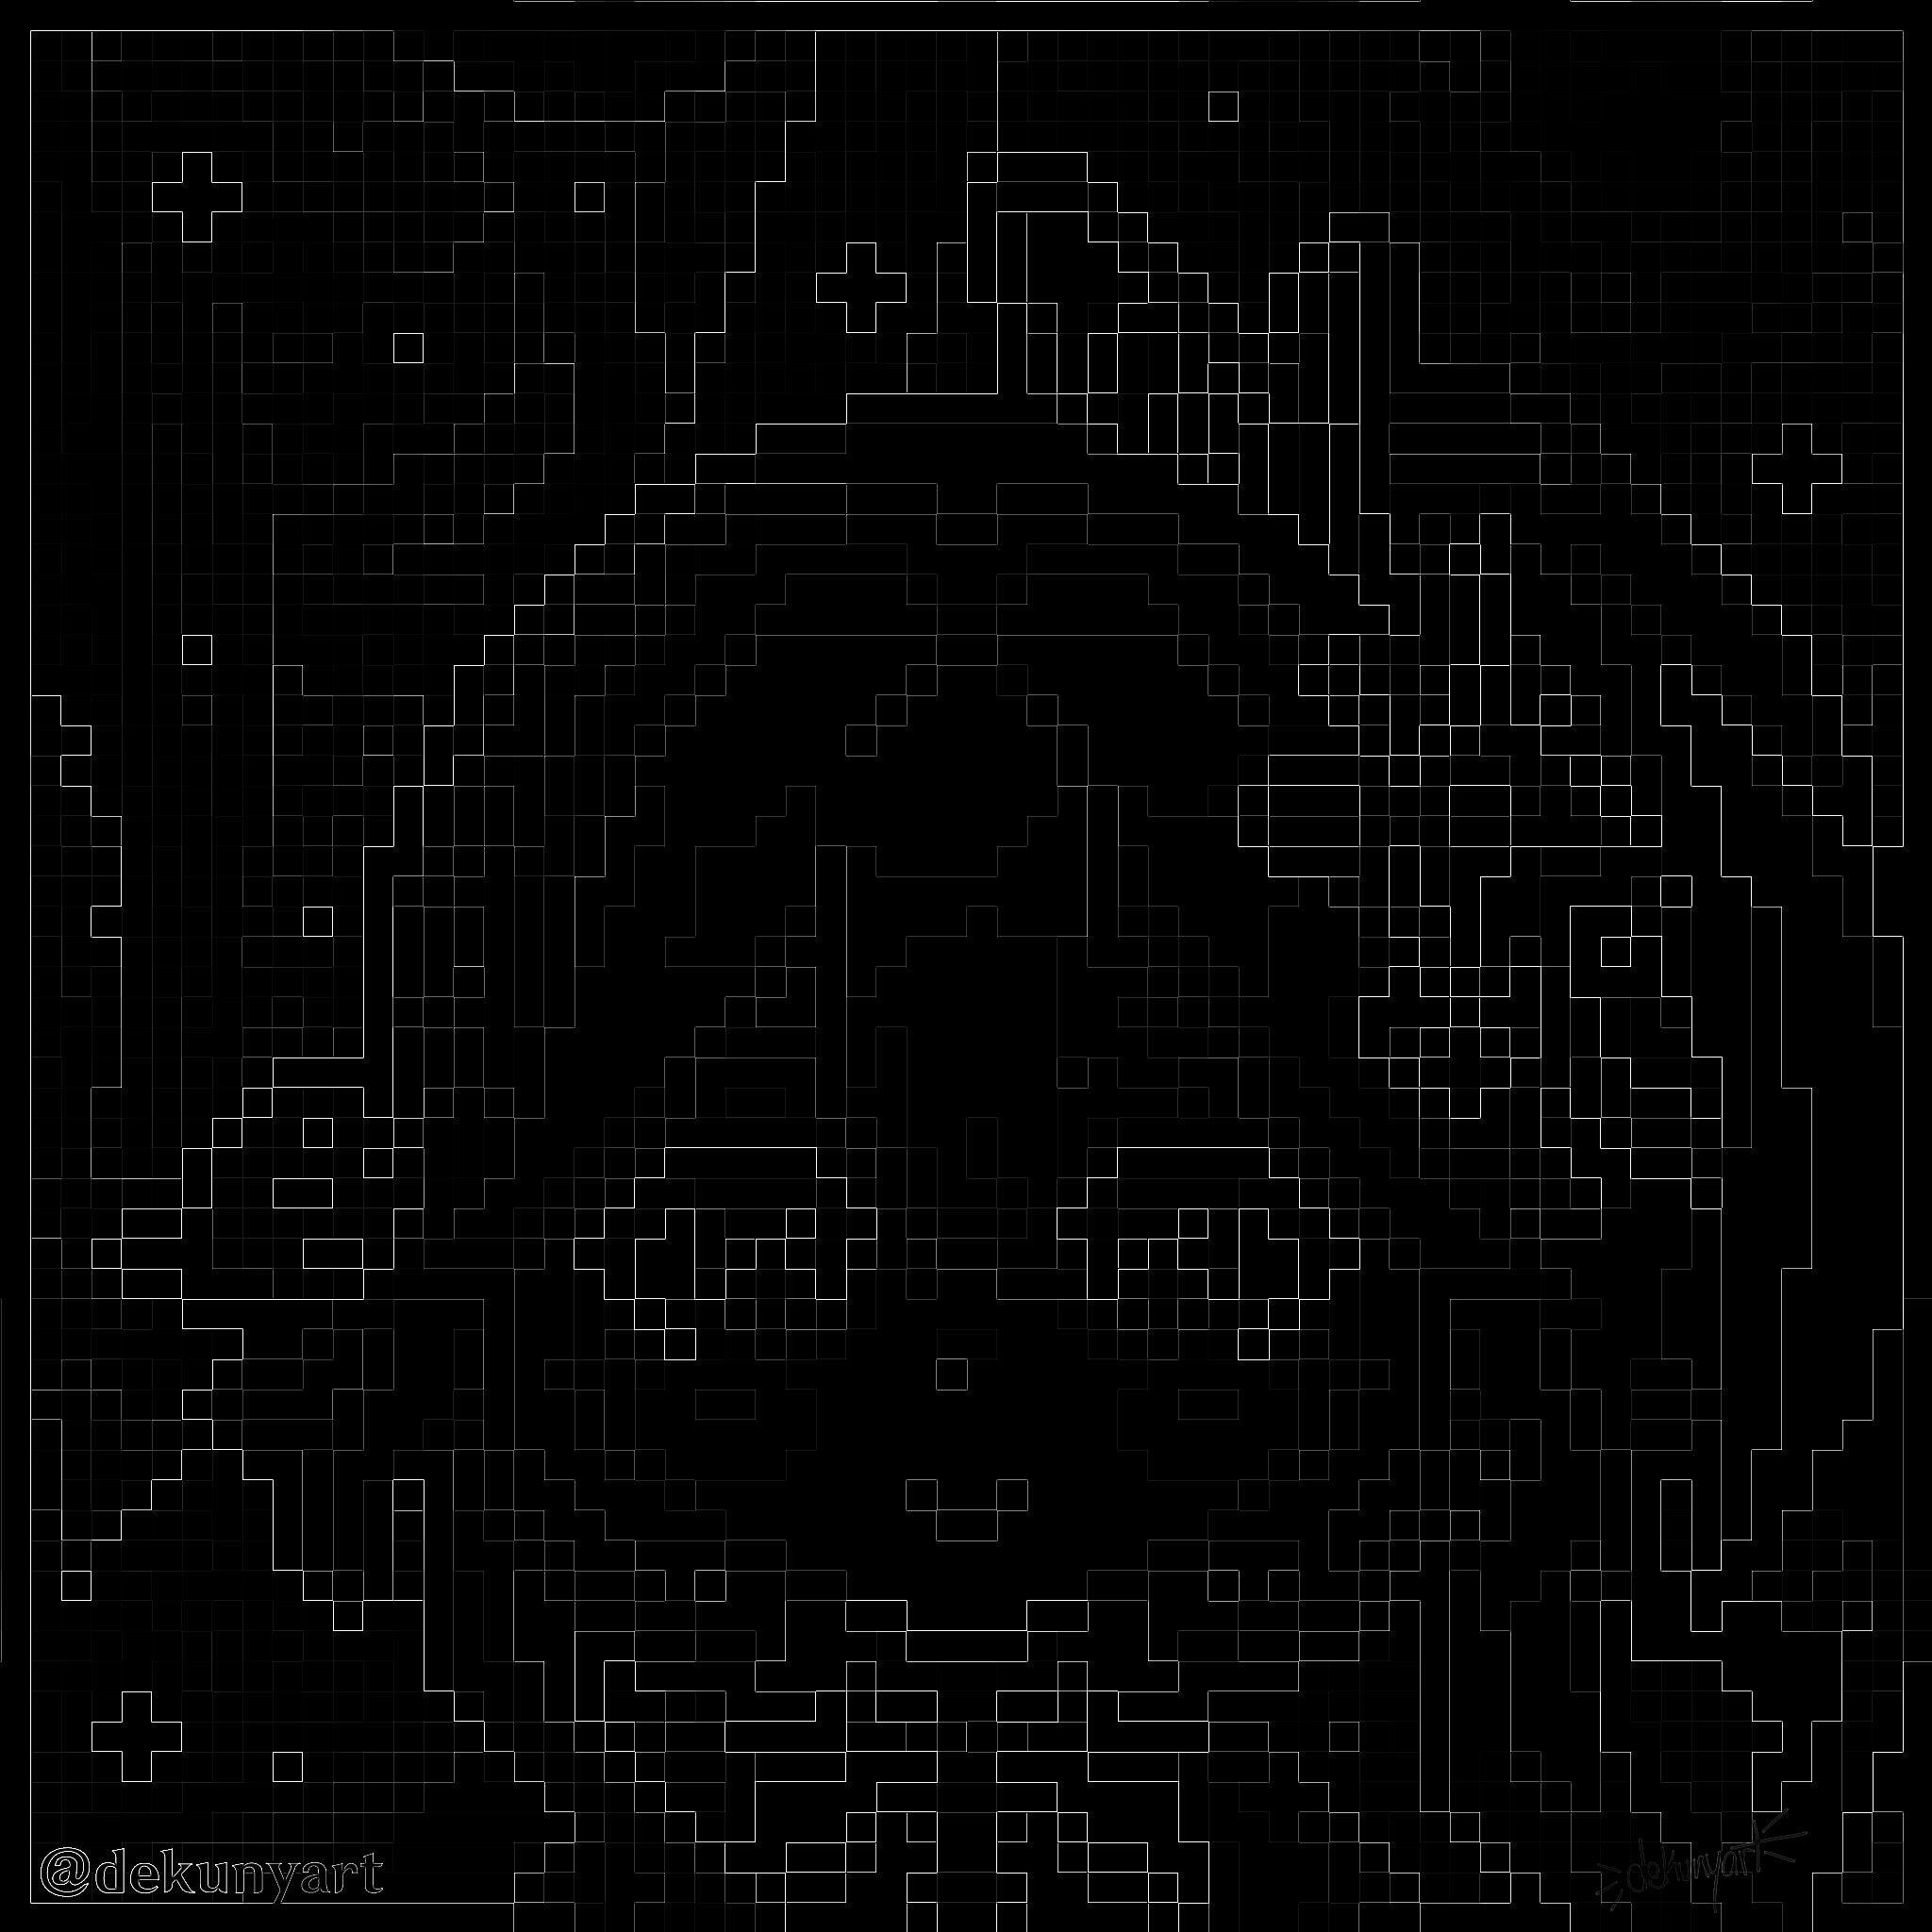
\includegraphics[width=0.6\textwidth]{pixel_art2_EDGE1.png}
	\caption{Выделяем края, применили один раз}
\end{figure}



\begin{figure}[ht]
    \centering
    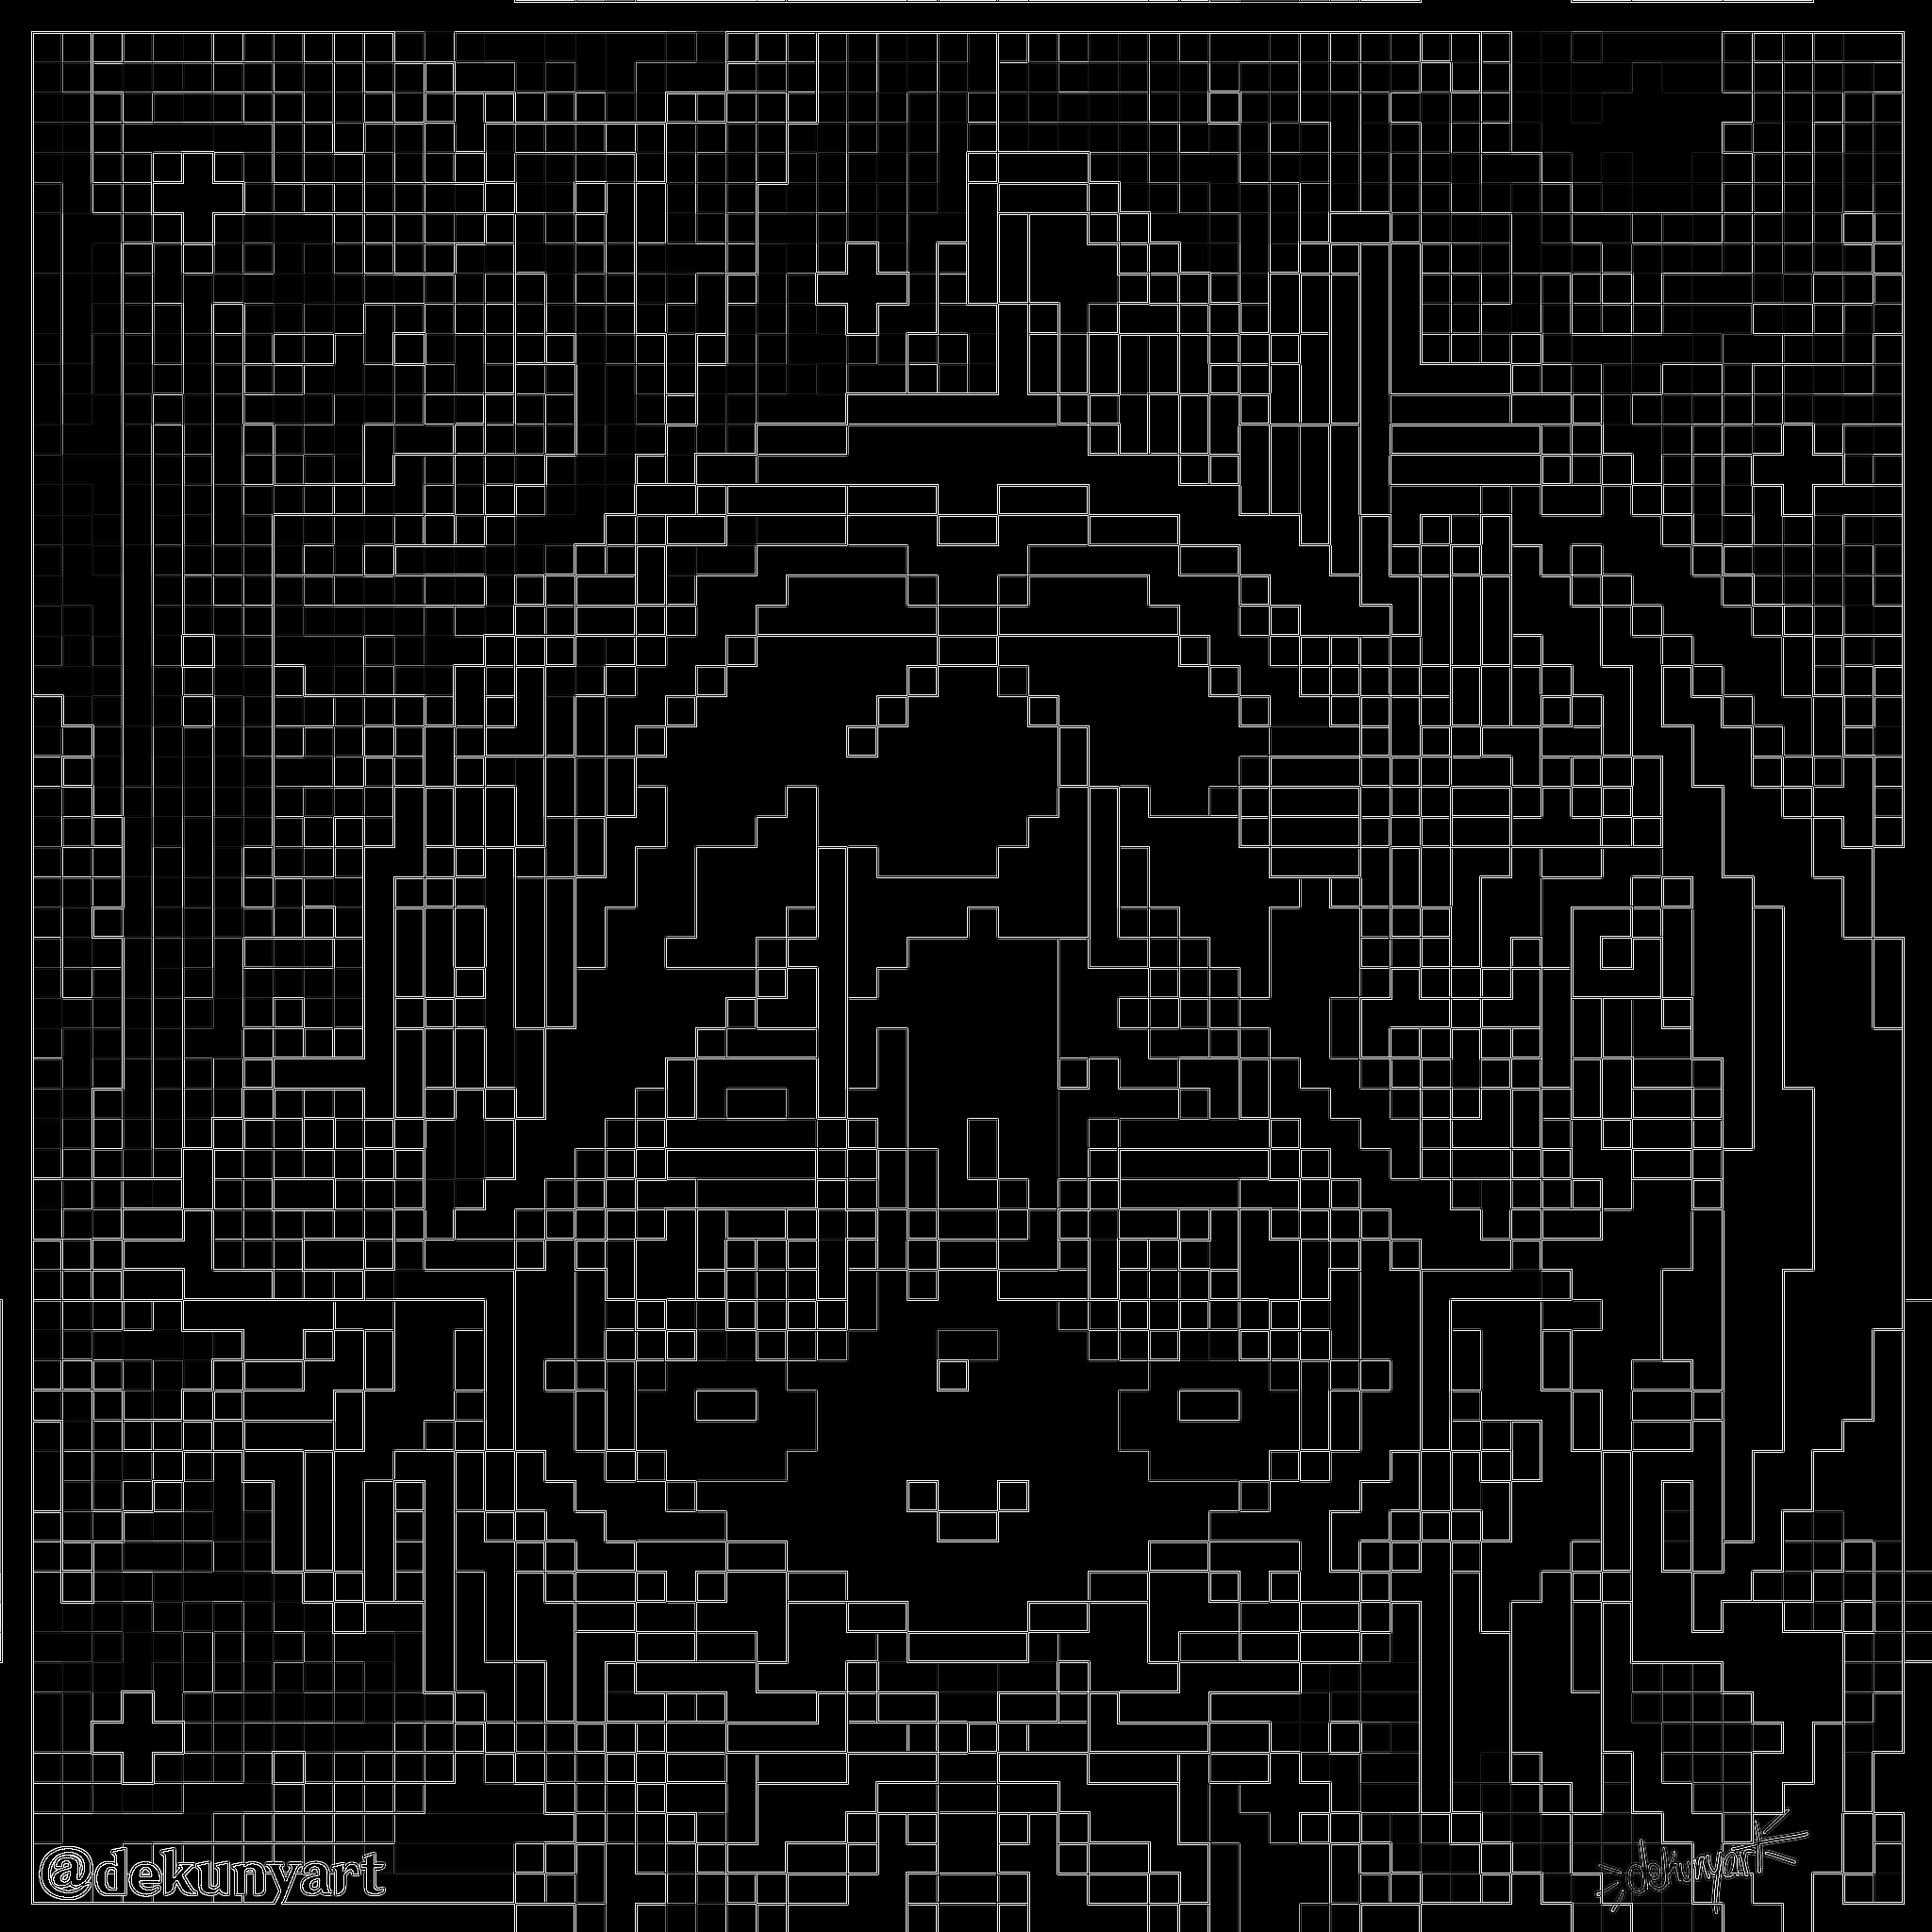
\includegraphics[width=0.6\textwidth]{pixel_art2_EDGE2.png}
	\caption{Выделяем края, применили два раза}
\end{figure}


\begin{figure}[ht]
    \centering
    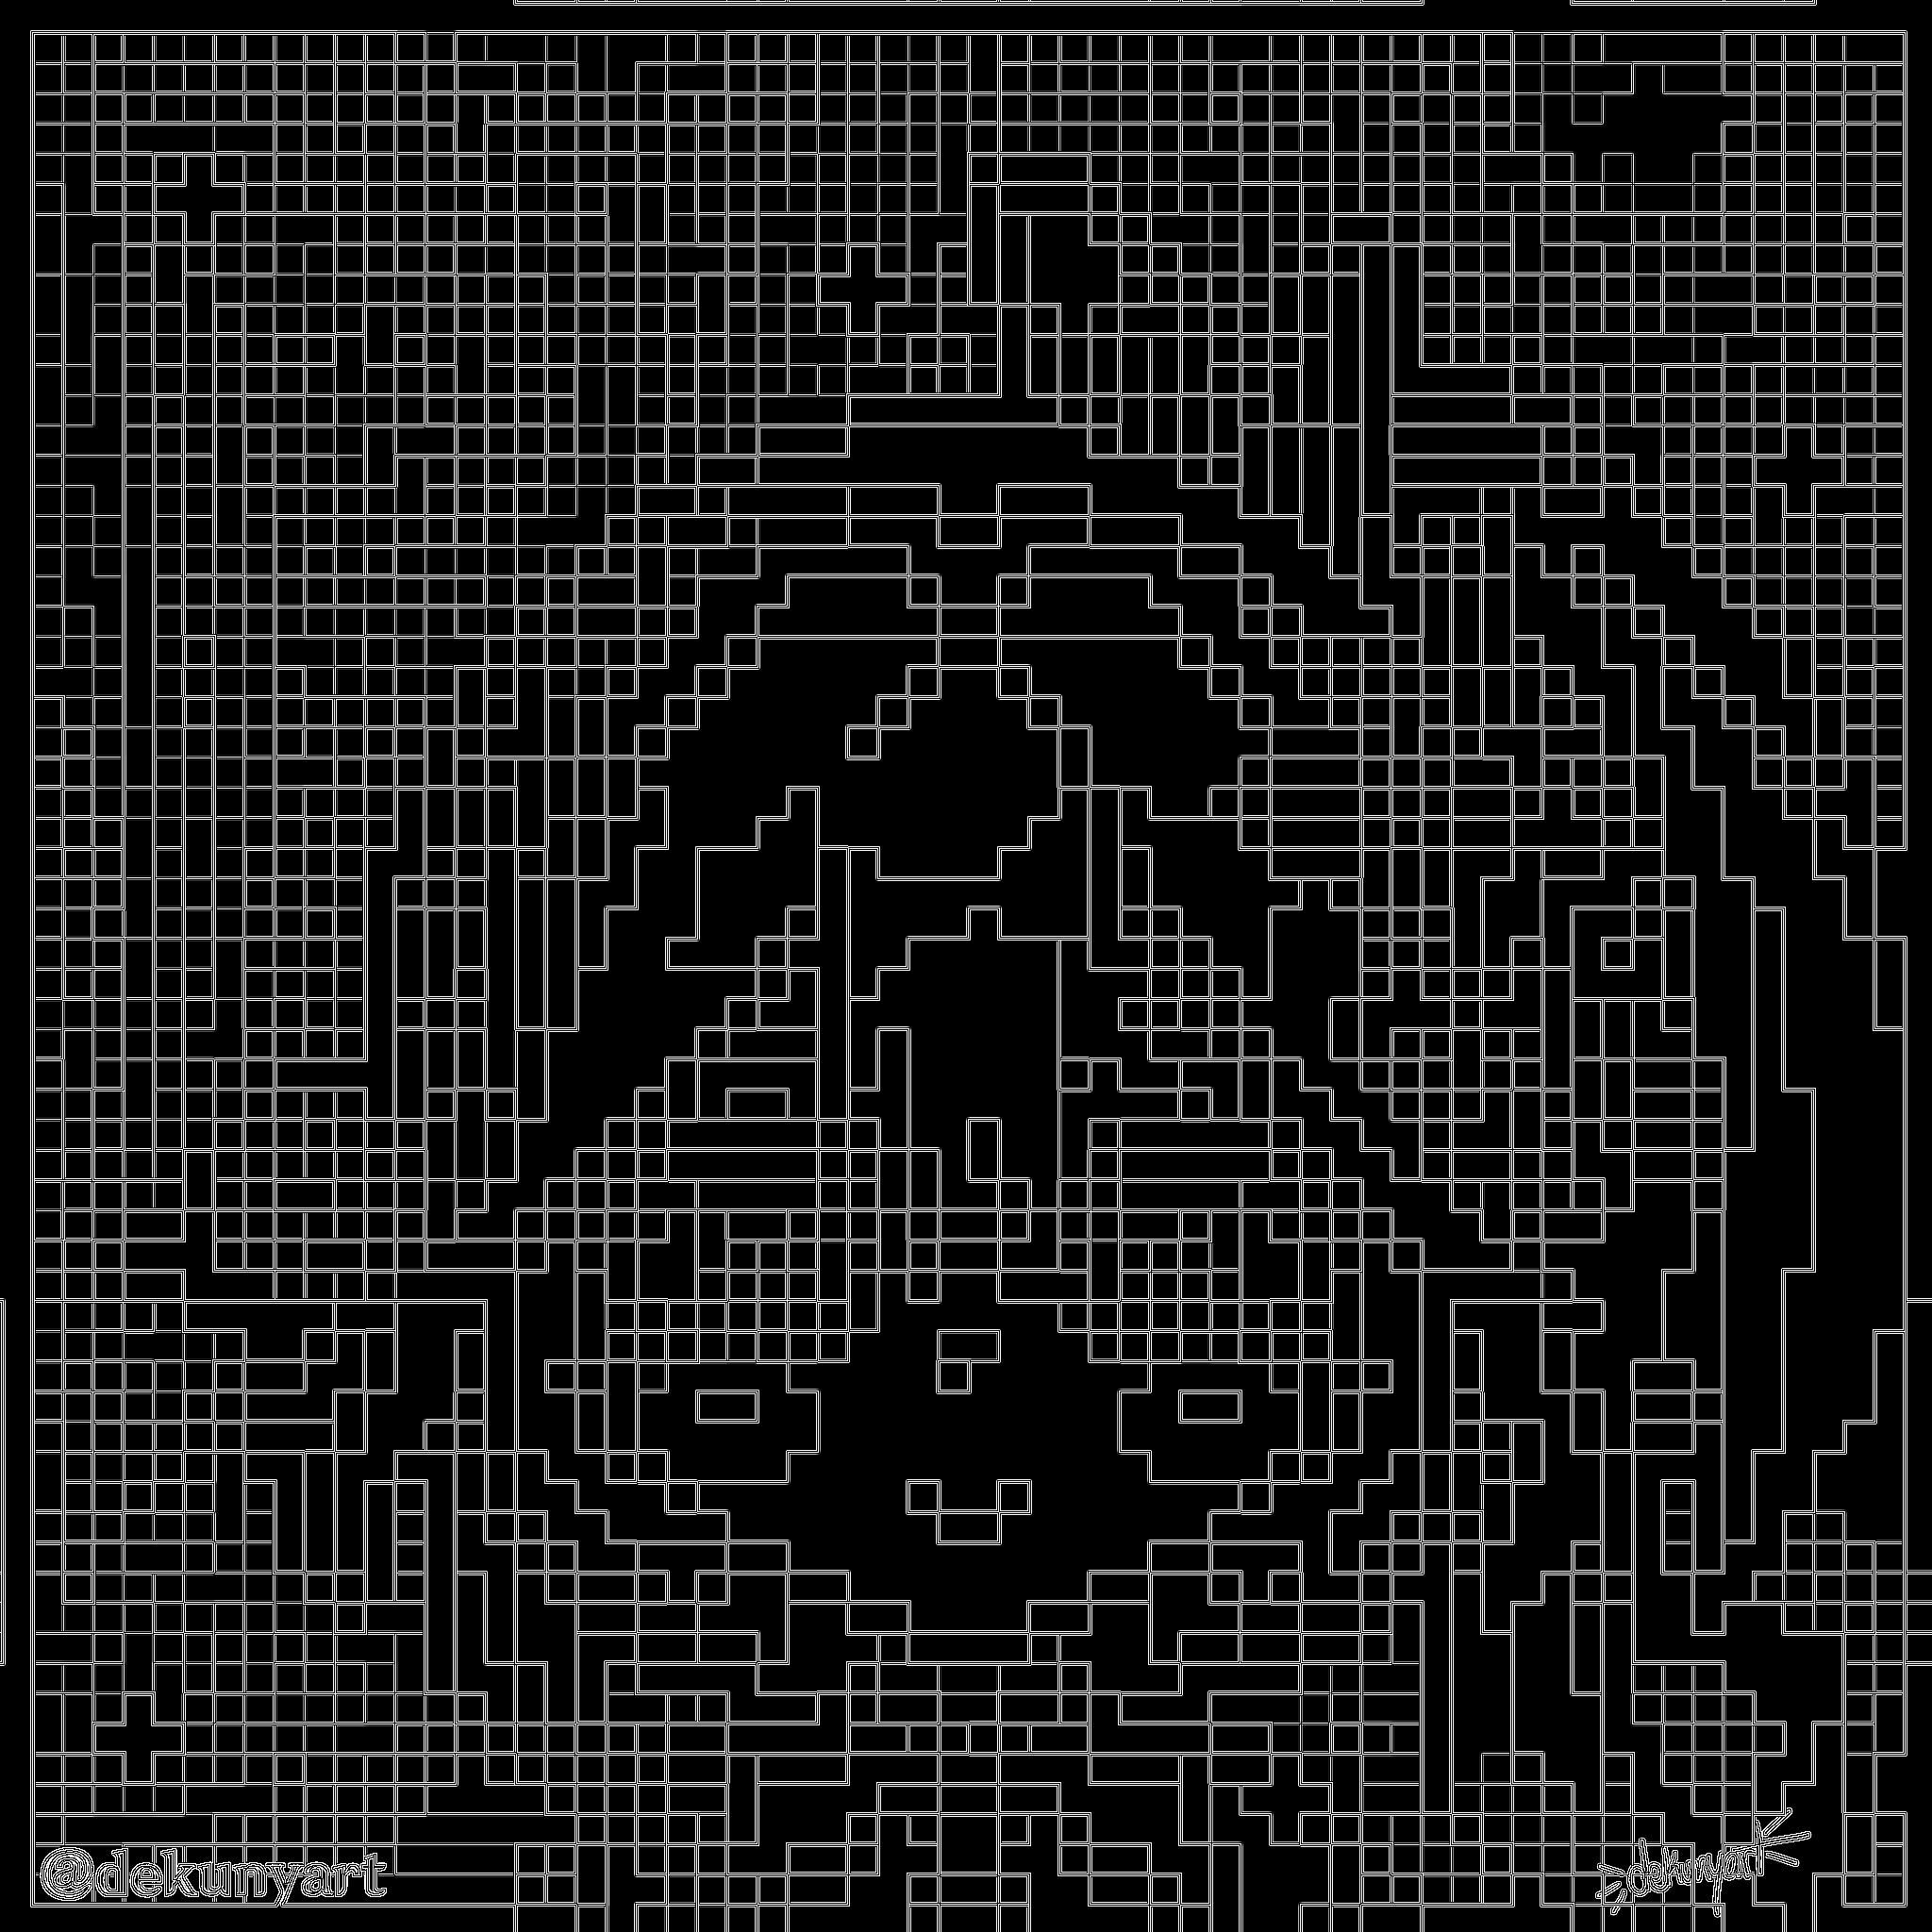
\includegraphics[width=0.6\textwidth]{pixel_art2_EDGE3.png}
	\caption{Выделяем края, применили три раза}
\end{figure}

\section{Мини-выводы}
Теорема о свёртке работает, ведь результаты двух разных подходов совпали\dots



\endinput